\documentclass[letterpaper, compsoc, conference]{IEEEtran}

\usepackage[ruled,vlined]{algorithm2e}
\usepackage{natbib}
\usepackage[cmex10]{amsmath}
\usepackage{array}
\usepackage[tight,footnotesize]{subfigure}
\usepackage[caption=false,font=footnotesize]{subfig}
\usepackage{url}
\usepackage{paralist}
\usepackage{tikz}
\usepackage{fancyhdr}
\usepackage{multirow}
\usetikzlibrary{snakes}
\usetikzlibrary{patterns}
\usetikzlibrary{circuits}
\usetikzlibrary{arrows,shapes.geometric,shapes.gates.logic.US,shapes.gates.logic.IEC,calc}

\begin{document}
\title{A Co-operative Parallel SAT Solver Based on Message Passing}

\author{
    \IEEEauthorblockN{Nayden Nedev}
    \IEEEauthorblockA{
        Department of Computer Science  \\
        Princeton University \\
        \textit{nnedev@cs.princeton.edu}
    } 
    \and \IEEEauthorblockN{Pramod Subramanyan}
    \IEEEauthorblockA{
        Department of Electrical Engineering \\
        Princeton University \\
        \textit{psubrama@princeton.edu}
    } 
}
\maketitle

\begin{abstract}
The Boolean Satisfiability Problem is a task with many practical applications
and is known to be NP-complete. Numerous different algorithms have been
proposed in the literature that effectively solve real-world instances of the
problem in a reasonable amount of time. 

With the advent of fast modern multiprocessor systems, new directions for
further improvement of the existing solutions arise. In this paper we present a
parallel SAT solver algorithm based on conflict-driven clause sharing and
message passing. We evaluate our approach on the base of the popular sequential
MiniSAT solver and compare it with one of the most successful parallel solvers
- ManySAT. Our experiments show that the proposed approach achieve up to 164
times speedup on some instances when run on a modern multicore architecture.

\end{abstract}

\section{Introduction}

The Boolean Satisfiability Problem, usually called just the SAT problem, is the
task of finding an assignment of all variables of a boolean formula such a way
that the whole formula evaluates to a true value.

The SAT problem has been thoroughly investigated and understood during the last
several decades. A lot of work has been done in both investigating the
theoretical properties of the problem and its practical implications. It is the
first problem in computer science that has been classifies as NP-complete
\cite{SATNP}. One of the reasons, because of which it is so important, is the
fact that many natural decision and optimizations problems in different areas
of science can be modelled as an instance of SAT. This resulted in extensive
research in this area and a lot of progress in finding efficient ways to solve
SAT in a reasonable amount of time. A myriad of different algorithms has
appeared in the scientific literature. Also, special competitions
\cite{SATComp} has been organized to compare different ideas and
implementations.

Most modern SAT solvers are entirely sequential and do not try to introduce any
kind of parallel computation in their algorithms. The rise of new powerful
multiprocessor architectures brings new directions in which SAT solvers can be
improved. In this paper, we propose a new parallel algorithm for solving the
SAT problem based on message passing techniques.

The rest of this paper is organized as follows: we make a review 
of the related work in Section 2, describe our solution in more detail in 
Section 3, present the preliminary results of it in Section 4 and 
conclude in Section 5.

\section{Related Work}
There are hundreds of different algorithms and their variations that have been
proposed for this problem. Basically, there are two main classes of modern
algorithms that are used to solve the SAT problem in practice: the
conflict-driven clause learning algorithm and the stochastic local search
algorithms. In the last years, parallel modifications of this approaches have
been proposed.

\subsection{Sequential Approaches}

This section provides a brief review of the advances in sequential SAT solvers.

\subsubsection{Davis-Putnam-Logemann-Loveland (DPLL)}

The DPLL algorithm, which is one of the first algorithmic techniques to solve
the problem of Boolean satisfiability is a complete search algorithm based on
back-tracking. DPLL uses the following heuristics before each recursive call:

\begin{itemize}
\item \textbf{Unit Propagation}: if a clause contains only one literal, it can
be only satisfied by giving such a value to the this literal that make it true. 

\item \textbf{Pure Literal Elimination}: if a variable occurs with only one
polarity in the whole formula, then it can be assigned with a value that
corresponds to this polarity.
\end{itemize}
These heuristics drastically reduce the search space.

\subsubsection{Conflict-Driven Clause Learning (CDCL)}

Conflict-driven clause learning (CDCL) was first proposed by the
GRASP~\cite{GRASP} solver. The key idea behind CDCL is that each time the
solver finds a part of search space that is unsatisfiable, it analyzes this
``conflict'' to learn a new clause. Keeping track of the \emph{learned clauses}
helps the solver from exploring the same ``dead-ends'' over and over again.

\subsubsection{Modern Solvers: Chaff and MiniSat} 
Chaff~\cite{CHAFF} improves upon GRASP using two techniques.  The first is a
data structure that enables efficient traversal of the clause database which is
required for unit propagation known as \textbf{Two-literal watching}.
Two-literal watching maintains the invariant that two unassigned variables are
watched in every clause. In other words, when a literal is assigned to, it is
removed from the watchlist and replaced with an unwatched literal. When no
unwatched literal can be found, it means the clause is eligible for unit
propagation. The key advantage of two-literal watching is that it enables
efficient unit propagation without requiring traversal of the entire clause
database.

The decision heuristic in a SAT solver determines which variable is to be
assigned to (``branched'' on) next.  \textbf{Variable State Independent
Decaying Sum (VSIDS)} was a decision heuristic instroduced by Chaff which tends
to make the SAT solver explore variables that were recently involved in
conflicts. VSIDS keeps track of an ``activity factor'' metric that is measure
of the number of recent conflicts a variable has been involved in.  The
intuition behind the metric is that it improves ``search space locality'' as
variables recently involved in conflicts are more likely to be chosen by the
decision heuristic.  This in turn improves overall performance by helping the
solver ``close-out'' large regions of the search space.

One of the main improvements that MiniSat~\cite{MiniSat} made on Chaff was
to exploit input pre-processing. We use MiniSat version 2.2 as the
baseline for our work.

\subsubsection{Stochastic Local Search Algorithm}
Another popular approach is to apply local search in the space of possible
assignments such, i.e. iteratively improving the current solution of the
problem with respect to some heuristic until all the constraints are satisfied.
The most successful SAT solvers based on this technique are WalkSAT
\cite{WalkSAT} and GSAT \cite{GSAT}.

\subsection{Parallel Approaches}
In contrast to the sequential solvers, a relatively small number of 
high-performance parallel approaches have been proposed.

\indent The earliest attempt for a parallel solver is PSATO \cite{PSATO}. It tries
to parallelize the sequential SATO (SAtisfiability Testing Optimized) solver
\cite{SATO}. Both versions use trie to represent the boolean formula. The exploration
of the search space is organized in master/slave model.

\indent A couple of algorithms - GrADSAT \cite{GRADSAT} and \cite{Blochinger} -
try to improve the successful sequential Chaff \cite{CHAFF}.

\indent The most recent notable parallel algorithm is ManySAT \citep{ManySAT}.
ManySAT uses a portfolio of complimentary sequential algorithms that are derived
from variations of the traditional DPLL algorithm. Each sequential algorithm shares
clauses, which leads to some additional improvement.

\section{Parallelization Strategy}
Our general strategy for parallelization is twofold. To a limited extent we use
divide and conquer strategy to ensure that the different processes are working
on different parts of the search space. However, processes co-operate with each
process by sharing learnt clauses with other processes. 

\subsection{Clause Sharing}

As the SAT solver explores the search space, it finds that certain regions of
the space are unsatisfiable. This occurs each time the solver runs into a
``conflict''. Modern solvers since GRASP~\cite{GRASP} \emph{analyze} each
conflict to learn clauses that ensure that ``dead-ends'' are never visited
again. In our solver, as in ManySAT~\cite{ManySAT}, clauses learnt by one
process are broadcast to all the other processes. This benefits speedup by
because clauses learned ensure that no other process visits that part 
of the search space again.

\subsubsection{What Clauses To Share}

One important design decision here is deciding which clauses are to be shared
with the other processes. As our results will show, sharing everything is not
feasible because the communication overhead outweighs any performance benefits
this may result in. Hammadi et al. \cite{Hammadi} suggest sharing clauses which
contain no more than a certain number of literals. The intuition here is that
short clauses are more ``general'', while long clause are more ``specific''.
Hence, sharing short clauses is likely to be useful to processes regardless of
what part of the search space they are in. In contrast, long clauses are likely
to be useful to processes only if they are exploring the same part of the
search space. 

Note the SAT solver will most likely \textit{not} explore all parts of the
search space as this would simply take too long. Modern solvers are efficient
because they determine satisfiability by using heuristics to explore only
those parts of the search space that are likely to lead to a solution.

\subsubsection{Clause Sharing Based on Activity Factors}

Modern solvers chose to explore parts of the search space determined by
variables with a high activity factor.  If two processes are exploring
``nearby'' parts of the search space, they will likely have the same set of
variables with high activity factors. This suggests that activity factors may
be a useful measure to determine which clauses ought to be shared with which
variables. The challenge here is in communicating the activity factors from one
process to another without the communication overhead negating any performance
gains that may result from the clause sharing.

One of the goals of our project is to gain an understanding of what clauses
would be useful to share and design mechanisms for ``intelligent'' learned
clause sharing.  Activity factors are likely to be a useful metric in designing
such mechanisms.

\subsection{Decision Heuristic} 

The decision heuristic in a SAT solver determines which variable is to be
assigned to and ``branch'' on next. Modern SAT solvers use the activity factor
metric to determine which variable to branch on.

Our parallel SAT solver has to balance the competing interests of dividing the
search space among different processes while ensuring that they don't go too
``far away'' from each other. If the processes are exploring completely
independent parts of the search space, the learned clauses from one process
will likely not be useful to other processes. 

Our current decision heuristic balances these goals in the following way.  If
two variables have exactly the same activity factor, the heuristic biases
process $i$ towards variables $v_k$ such that $k~mod~i=0$. If two variables
have differing activity factors, the ``default'' heuristic of preferring the
higher activity variable is used.

It is possible that if two variables similar but not equal activity factors, it
might still be beneficial to bias certain threads towards certain variables. We
intend to examine the impact of this type of decision heuristic in the final
submission.

\subsection{A Clustered Approach}


\section{Results}

The section describes our preliminary results with the simple clause sharing
technique described earlier. The results shown in Section \ref{sec:speedup}
share clauses with 16 literals or fewer with all the other cores. Section
\ref{sec:sharing effects} investigates the impact of sharing shorter
and longer clauses.

\subsection{Methodology}
Our benchmark problems are taken from SAT-Race 2008~\cite{SATRace2008}. We
executed all 100 problems used in the competition using the sequential SAT
solver MiniSat 2.2 with a time limit of 5 minutes.\footnote{MiniSat 2.1 was the
fastest solver in SAT-Race 2008} Among these 100 problems, we chose to
experiment with a subset of 25 problems that took MiniSat 2.2 between 40s and
200s to execute. Our intention in choosing this subset was to choose a small
number of problems that we could execute relatively quickly and often while
simultaneously ensuring that we avoid those that finished in a few seconds.  We
intend to present full results in the standard SAT-Race format (time limit of
15 minutes) for the final submission of this report.

Fourteen among the chosen 25 problems were satisfiable while the remaining
eleven were unsatisfiable.

Experiments were performed on an 8-core Intel\textregistered
~Xeon\textregistered ~E31230 CPU clocked at 3.20GHz with 32 GB of RAM. The
comparison with ManySAT uses ManySAT version 2.0 obtained
from~\cite{ManySATWeb}.  The default command-line and default parameter
settings were used when executing ManySAT.


\subsection{Speedup}
\label{sec:speedup}

\begin{table*}[htbp]
    \begin{center}
    \begin{tabular}{|l|c|c|c|c|c|c|c|c|}
        \hline
        {\textbf{SAT Benchmark}} & \multicolumn{4}{c|}{\bf ManySAT 2.0} & \multicolumn{4}{c|}{\bf MPI-based Parallel Solver} \\
        \hline
        & $n=1$ & $n=2$ & $n=4$ & $n=8$ & $n=1$ & $n=2$ & $n=4$ & $n=8$ \\
        \hline
        ibm-2004-29-k25                          &    1.0 &    0.7 &    0.7 &    0.3 &    1.0 &    1.1 &    2.5 &    2.9 \\
        ibm-2004-1\_11-k80                       &    1.0 &    0.3 &    0.2 &    0.1 &    1.0 &    0.7 &    0.8 &    1.1 \\
        ibm-2002-20r-k75                         &    1.0 &    0.6 &    0.5 &    0.1 &    1.0 &    1.1 &    2.6 &    1.7 \\
        simon-s02b-r4b1k1.2                      &    1.0 &    1.7 &    1.2 &    5.9 &    1.0 &   25.7 &   22.6 &    3.3 \\
        velev-npe-1.0-9dlx-b71                   &    1.0 &    0.2 &    0.2 &    0.1 &    1.0 &    3.7 &    1.7 &    1.6 \\
        schup-l2s-motst-2-k315                   &    1.0 &    0.4 &    0.3 &    0.2 &    1.0 &    0.5 &    1.1 &    0.8 \\
        goldb-heqc-alu4mul                       &    1.0 &    1.0 &    0.7 &    0.3 &    1.0 &    1.9 &    3.3 &    3.0 \\
        jarvi-eq-atree-9                         &    1.1 &    0.8 &    0.7 &    0.9 &    1.0 &    1.2 &    2.5 &    2.0 \\
        ibm-2002-22r-k80                         &    1.0 &    0.3 &    0.6 &    0.1 &    1.0 &    0.5 &    1.0 &    1.8 \\
        simon-s03-fifo8-400                      &    1.0 &    0.9 &    0.4 &    0.2 &    1.0 &    1.8 &    1.9 &    2.2 \\
        ibm-2002-24r3-k100                       &    1.0 &    1.0 &    0.5 &    0.3 &    1.0 &    1.8 &    2.3 &    3.0 \\
        mizh-sha0-36-4                           &    1.0 &    1.2 &    1.0 &    0.4 &    1.0 &    0.2 &    0.8 &    0.6 \\
        manol-pipe-f7nidw                        &    1.0 &    0.9 &    0.6 &    0.2 &    1.0 &    1.6 &    2.3 &    2.4 \\
        manol-pipe-c6bidw\_i                     &    1.0 &    0.6 &    0.4 &    0.2 &    1.0 &    1.5 &    1.6 &    2.0 \\
        mizh-md5-47-3                            &    1.0 &    0.3 &    0.3 &    0.2 &    1.0 &    1.4 &    2.3 &    5.6 \\
        ibm-2004-23-k80                          &    1.0 &    0.5 &    0.2 &    0.1 &    1.0 &    0.7 &    1.1 &    3.5 \\
        mizh-md5-48-2                            &    1.0 &    0.1 &    0.1 &    0.1 &    1.0 &    1.4 &    2.2 &    5.9 \\
        ibm-2002-22r-k75                         &    1.0 &    0.5 &    0.4 &    0.2 &    1.0 &    1.8 &    1.9 &    2.0 \\
        manol-pipe-g10nid                        &    1.0 &    0.7 &    0.4 &    0.2 &    1.0 &    1.3 &    1.8 &    1.6 \\
        fuhs-aprove-16                           &    1.0 &    0.4 &    0.3 &    0.2 &    1.0 &    1.0 &    1.7 &    1.7 \\
        post-c32s-col400-16                      &    1.0 &    0.6 &    0.4 &    0.3 &    1.0 &    1.5 &    2.1 &    2.3 \\
        anbul-dated-5-15-u                       &    1.0 &    0.9 &    0.6 &    0.3 &    1.0 &    2.0 &    2.0 &    1.7 \\
        mizh-sha0-35-4                           &    1.0 &    1.7 &    0.6 &    0.4 &    1.0 &    5.9 &    1.6 &    9.0 \\
        ibm-2004-29-k55                          &    1.0 &    7.1 &    5.0 &    1.9 &    1.0 &   21.5 &  164.3 &   59.2 \\
        mizh-sha0-36-1                           &    1.0 &    0.3 &    0.3 &    0.5 &    1.0 &    0.6 &   11.2 &   14.6 \\
        \hline
    \end{tabular}
    \end{center}
    \caption{Speedup of parallel SAT solvers as $n$ (number of cores) is
    varied. Speedup is computed using MiniSat 2.2 as the baseline. }
    \label{tab:speedup}
\end{table*}
Table \ref{tab:speedup} shows the speedup of the ManySAT 2.0 and our
implementation for the 25 selected benchmarks. Speedups are shown for 1, 2, 4
and 8 cores. Somewhat surprisingly, ManySAT 2.0 does not show significant
speedup for most of the benchmarks. We are trying to understand why this
is the case.

Our implementation shows significant speedup ($>2X$) when using 4 cores and
slightly more than that for 8 cores. Since learnt clauses are broadcast
to all the other cores, it would seem that communication overheard for 8
cores outweighs the sharing benefit.

\begin{figure}[htbp]
    \begin{center}
        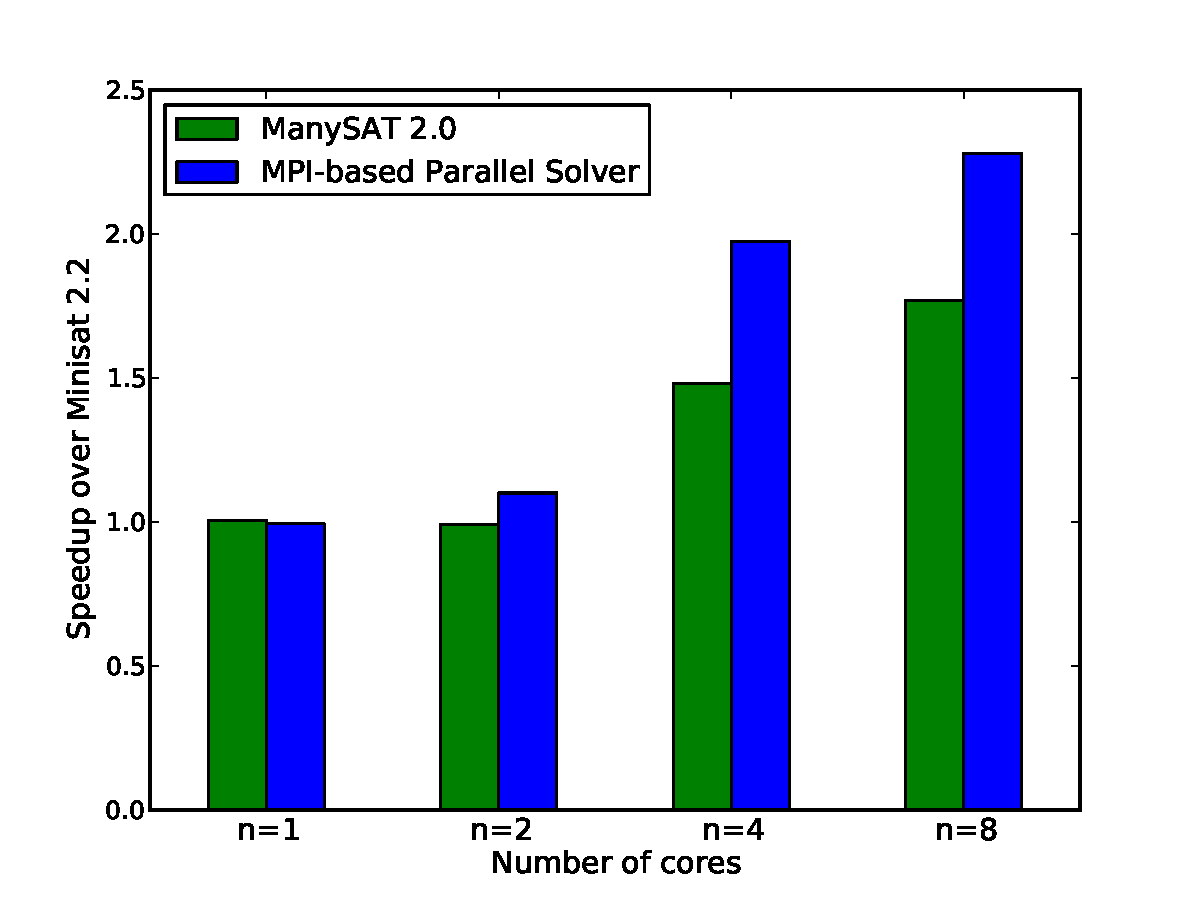
\includegraphics[width=\columnwidth]{images/speedup1.pdf}
        \caption{Overall Execution Speedup.}
        \label{fig:speedup}
    \end{center}
\end{figure}

Figure \ref{fig:speedup} presents the \emph{overall execution speedup} for the
problems shown in Table \ref{tab:speedup}. The overall speedup measured here is
speedup compared to MiniSat 2.2 baseline for the time taken to solve all 25
problems by the two parallel solvers. It can be seen that the MPI-based
parallel solver gets only slightly faster when going from 1 to 2 cores. Going
from 2 to 4 cores produces significant speedup but speedup is already tapering
off at 8 cores.

\subsection{Effect of Clause Sharing}
\label{sec:sharing effects}

\begin{figure}[htbp]
    \begin{center}
        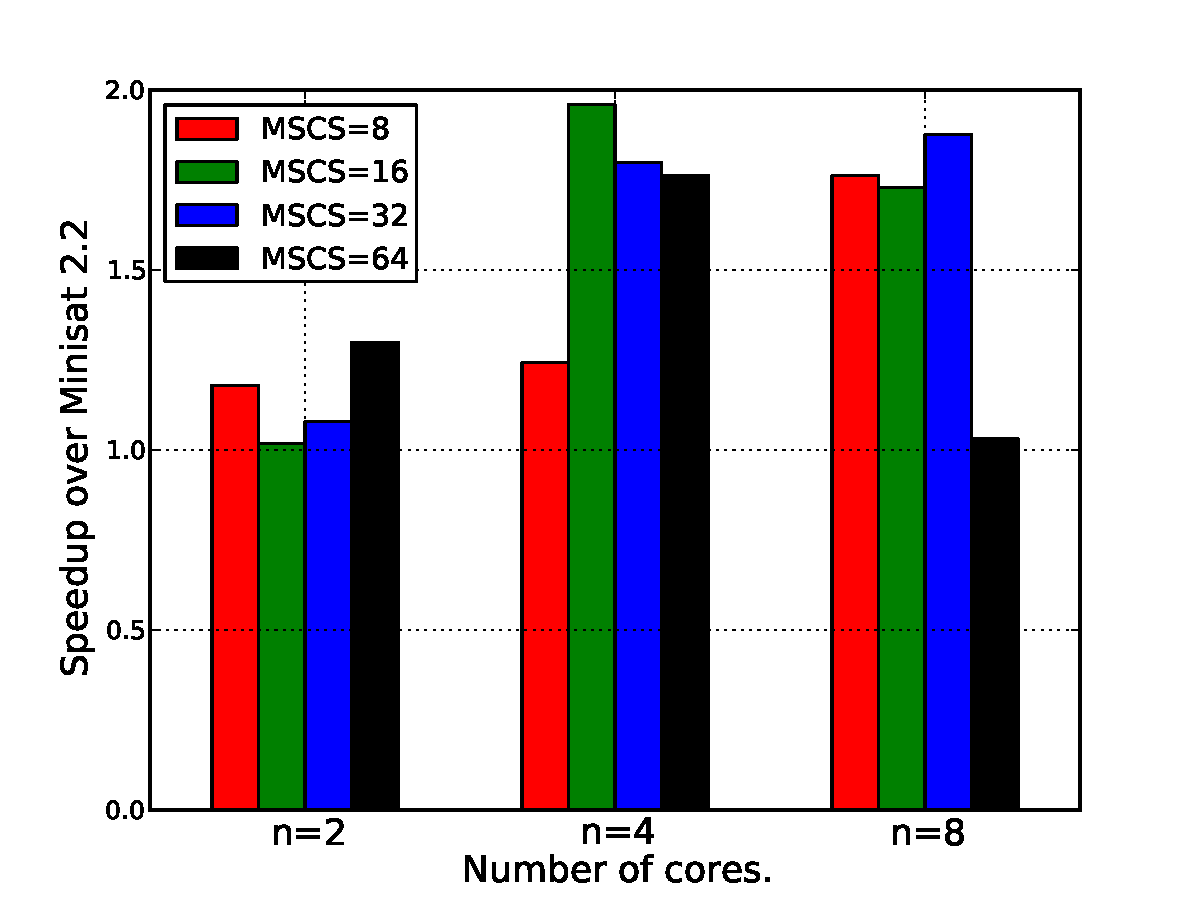
\includegraphics[width=\columnwidth]{images/mcs.pdf}
        \caption{Effect of maximum shared clause size (MSCS).}
        \label{fig:mscs}
    \end{center}
\end{figure}

Figure \ref{fig:mscs} shows the effect of maximum size of shared clauses on the
speedup. Note these results are slightly different from those shown in Figure
\ref{fig:speedup} because of noise in the timing measurements. Although the
trends are somewhat hard to interpret because of the noise, some observations
that can be made are the following.

\begin{enumerate}

\item When executing with only 2 cores, sharing as many clauses as possible
(i.e., up to maximum sharing clause size (MSCS) of 64) is beneficial.

\item When executing with four cores, the best performance is achieved when
MSCS=16. This number corresponds to the results shown in the previous
subsection.

\item When executing with either cores, sharing less (MSCS=8) seems to be the
best although there is an abberant data point for MSCS=32.
      
\end{enumerate}


\section*{Acknowledgements}

We would like to thank Professor David Wentzlaff and Professor Sharad Malik for
sharing their suggestions and ideas with us.

\section{Conclusion}

\bibliographystyle{plain}
\bibliography{report}
\end{document}
